% !TEX TS-program = pdflatex
% !TEX encoding = UTF-8 Unicode

\documentclass{beamer}

\mode<presentation>
{
  \usetheme{Montpellier}
  % or ...
  \usecolortheme{dolphin}
  \setbeamercovered{transparent}
  % or whatever (possibly just delete it)
}


\usepackage[english]{babel}
% or whatever



\usepackage[utf8]{inputenc}
% or whatever

\usepackage{times}
\usepackage[T1]{fontenc}
% Or whatever. Note that the encoding and the font should match. If T1
% does not look nice, try deleting the line with the fontenc.


\title[Web Service Pays] % (optional, use only with long paper titles)
{Web Service Pays}

\subtitle
{Projet Etamine}

\author{Quentin Amelot \and Damien Larminé \and Fayize Kaimou  \\ \and Gisio Tabera \and Jérémie Nizou \and Paul Baudouin}
% - Give the names in the same order as the appear in the paper.
% - Use the \inst{?} command only if the authors have different
%   affiliation.

\institute[Université Paris 13] % (optional, but mostly needed)
{Master 1 Informatique \\ Université Paris 13}
% - Use the \inst command only if there are several affiliations.
% - Keep it simple, no one is interested in your street address.

\date[C&P 17/04/2015] % (optional, should be abbreviation of conference name)
{Conduite et Gestion de projets}
% - Either use conference name or its abbreviation.
% - Not really informative to the audience, more for people (including
%   yourself) who are reading the slides online

\subject{Theoretical Computer Science}
% This is only inserted into the PDF information catalog. Can be left
% out. 



% If you have a file called "university-logo-filename.xxx", where xxx
% is a graphic format that can be processed by latex or pdflatex,
% resp., then you can add a logo as follows:

\pgfdeclareimage[height=0.8cm]{university-logo}{images/university-logo-filename}
\logo{\pgfuseimage{university-logo}}



% Delete this, if you do not want the table of contents to pop up at
% the beginning of each subsection:
\AtBeginSubsection[]
{
  \begin{frame}<beamer>{Web Service}
    \tableofcontents[currentsection,currentsubsection]
  \end{frame}
}


% If you wish to uncover everything in a step-wise fashion, uncomment
% the following command: 

%\beamerdefaultoverlayspecification{<+->}


\begin{document}

\begin{frame}
  \titlepage
\end{frame}

\begin{frame}{Web Service}
  \tableofcontents
  % You might wish to add the option [pausesections]
\end{frame}


% Structuring a talk is a difficult task and the following structure
% may not be suitable. Here are some rules that apply for this
% solution: 

% - Exactly two or three sections (other than the summary).
% - At *most* three subsections per section.
% - Talk about 30s to 2min per frame. So there should be between about
%   15 and 30 frames, all told.

% - A conference audience is likely to know very little of what you
%   are going to talk about. So *simplify*!
% - In a 20min talk, getting the main ideas across is hard
%   enough. Leave out details, even if it means being less precise than
%   you think necessary.
% - If you omit details that are vital to the proof/implementation,
%   just say so once. Everybody will be happy with that.

\section{Le Web Service}

\subsection{Qu'est-ce qu'un web service ?}

\begin{frame}{Qu'est-ce qu'un web service ?}
  % - A title should summarize the slide in an understandable fashion
  %   for anyone how does not follow everything on the slide itself.

  \begin{itemize}
  \item
   Permet l'échange des données dans un environnement distribué.
  \item
    Ensemble de fonctionnalités pour des machines.
  \item
    Pas d'intervention humaine.
  \end{itemize}

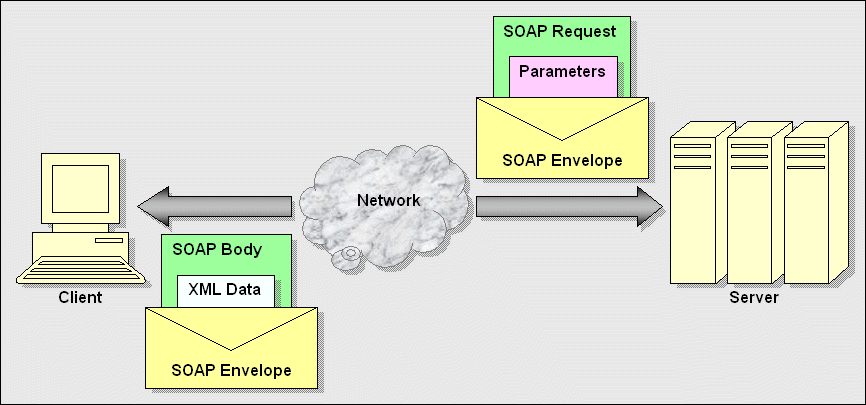
\includegraphics[scale = 0.25]{images/WS}

\end{frame}

\begin{frame}{Différentes technologies}

   2 technologies principales pour les web services :
  \begin{description}
    \item[SOAP] Fonctionnalités accessibles via un modèle de données décrit dans un fichier XML.
      \pause
    \item[REST] Fonctionnalités accessibles via la syntaxe du protocole HTTP.
  \end{description}
\end{frame}


\subsection{Notre projet}

\begin{frame}{Origine du projet}
\begin{itemize}
  \item
     Étamine
	\begin{itemize}
   	\item
      	Mutualiser des informations exhaustives dans une grande quantité de domaines.
	\end{itemize}
   \pause
   \item
      Notre projet
	\begin{itemize}
	\item
   	  Réalisation d'un web service permettant d'accéder aux informations des pays.
	\end{itemize}
\end{itemize}
\end{frame}

\begin{frame}{Pourquoi un web service ?}

\begin{itemize}
\item 
  Absence d'intervention humaine
  \pause
\item
  Automatisation et optimisation des tâches
  \pause
\item 
  Facilité d'intégration à Étamine
\end{itemize}

\end{frame}

\section{Développement du projet}

\subsection{Réalisation}

\begin{frame}{Débuts du projet}
\begin{itemize}
  \item
    Découverte du projet et des technologies nécessaires.
  \item
    Tutoriels et exemples sur Internet pour appréhender le sujet.
\end{itemize}
\end{frame}

\begin{frame}{Débuts de la programmation}
\begin{itemize}
  \item
    Programmation de l'application principale : le web service.
  \item
   Priorité sur cette aplication et mise au second plan des autres logiciels.
  \item
   Nombreuses réunions avec le client.
\end{itemize}
\end{frame}

\begin{frame}{Déroulement du projet}
\begin{itemize}
  \item
    Développement des clients après le web service.
  \item
    Mise à jour de la base de données.
  \item
    Finalisation des applications et développement de l'application de gestion.
\end{itemize}
\end{frame}


\subsection{Choix Techniques}

\begin{frame}{Technologies Principales}
\begin{itemize}
  \item JAVA
     \begin{itemize}
        \item
        	Langage multiplate-forme et facile d'accès.
        \item
	IDE utilisé : NetBeans 8.0.
     \end{itemize}
  \item Spring et Spring-WS
    \begin{itemize}
      \item
       Framework souple et puissant.
    \end{itemize}
\end{itemize}

\end{frame}

\begin{frame}{Technologies de gestion et mise en place}
\begin{itemize}
  \item Maven
     \begin{itemize}
        \item
        	Outil de gestion de projets en Java.
     \end{itemize}
  \item Tomcat
    \begin{itemize}
      \item
       Serveur Java directement intégré à Spring. 
    \end{itemize}
\end{itemize}
\end{frame}

\begin{frame}{Autres Technologies}
\begin{itemize}
  \item \LaTeX
     \begin{itemize}
        \item
           Système de composition de documents utilisés pour la documentation.
     \end{itemize}
  \item Autres technologies
    \begin{itemize}
      \item
       Frameworks Java : JAXB, JUnit, JDBC
     \item
       Technolgie SOAP et SoapUI
    \end{itemize}
\end{itemize}
\end{frame}

\section{Difficultés Rencontrées}

\subsection{Technologies inconnues}

\begin{frame}{Technologies inconnues}
\begin{itemize}
  \item Prise en main difficile :
     \begin{itemize}
          \item Technologies enseignées en Master 2.
          \item Apprentissage nécessaire.
    \end{itemize}
\end{itemize}
\end{frame}

\subsection{Complications durant le développement}

\begin{frame}{Complications durant le développement}
\begin{itemize}
  \item Petites difficultés facilement corrigibles.
  \item Aucune grosse complication durant le développement.
\end{itemize}
\end{frame}

\section*{Conclusion}

\begin{frame}{Conclusion}

  % Keep the summary *very short*.
  \begin{itemize}
  \item
    Projet intéressant et utile.
  \item
    Bonne entente, groupe travailleur.
  \item
    Possibilités d'améliorations pour le projet.
  \end{itemize}
  
\end{frame}

\begin{frame}
  \frametitle<presentation>{Remerciements}
	\vspace*{\fill}
	\begin{center}
	\begin{minipage}{.6\textwidth}
	\LARGE Merci de votre attention
	\end{minipage}
	\end{center}
	\vfill
\end{frame}


\begin{frame}
  \frametitle<presentation>{Informations Complémentaires}
    
     Pour plus d'informations :
  \begin{thebibliography}{10}
    
  \beamertemplateonlinebibitems
  % Start with overview books.

  \bibitem{Trac}
     Trac Wiki
    \newblock  https://trac.lipn.univ-paris13.fr/projects/pays/

  \bibitem{Site M.Fortier}
     Site de Mr Fortier
    \newblock {https://lipn.univ-paris13.fr/\textasciitilde fortier/Wiki/}
  \end{thebibliography}
\end{frame}

\end{document}


